%
% Modified by Megan Patnott
% Last Change: Jan 18, 2013
%
%%%%%%%%%%%%%%%%%%%%%%%%%%%%%%%%%%%%%%%%%%%%%%%%%%%%%%%%%%%%%%%%%%%%%%%%
%
% Modified by Sameer Vijay
% Last Change: Tue Jul 26 2005 13:00 CEST
%
%%%%%%%%%%%%%%%%%%%%%%%%%%%%%%%%%%%%%%%%%%%%%%%%%%%%%%%%%%%%%%%%%%%%%%%%
%
% Sample Notre Dame Thesis/Dissertation
% Using Donald Peterson's ndthesis classfile
%
% Written by Jeff Squyres and Don Peterson
%
% Provided by the Information Technology Committee of
%   the Graduate Student Union
%   http://www.gsu.nd.edu/
%
% Nothing in this document is serious except the format.  :-)
%
% If you have any suggestions, comments, questions, please send e-mail
% to: ndthesis@gsu.nd.edu
%
%%%%%%%%%%%%%%%%%%%%%%%%%%%%%%%%%%%%%%%%%%%%%%%%%%%%%%%%%%%%%%%%%%%%%%%%
%
% Chapter 1
%

%\documentclass{article}
%\usepackage{mathtools}

\chapter{INTRODUCTION}

In computer simulation of condensed phase molecular systems, molecules are commonly represented by atomic sites that interact via a parametrized force field. This force field aims to reproduce observable phenomena by incorporating the proper physics into the simulation. There are mainly two types of interaction; intramolecular and intermolecular which determines the static and dynamic properties of the molecular systems. An intramolecular interaction is the interaction within a single molecule including, bonding, bending, and torsional motion whereas an intermolecular interaction is the interaction between two or more molecules and includes van der Waals and electrostatic interactions. The computation of the electrostatic interaction is the most expensive portion of a molecular simulations. Due to this, there have been significant efforts to develop practical, efficient, and accurate methods for electrostatic interactions. 

The Ewald method is one of the most well known and accurate methods but is computationally expensive, scaling as O($N^2$), where $N$ is the total number of particles. The appropriate selection of a damping parameter and suitable algorithm can decrease computational cost to O($N^{3/2}$).\cite{Perram88} Modified Ewald methods, using a particle mesh and fast Fourier transform (FFT), have decreased the cost to O($N\log N$). \cite{Shimada93, Luty95, Darden93,Essmann95} But these modified Ewald methods (particle mesh Ewald (PME) and particle-particle particle-mesh Ewald (PPPME)) are still computationally expensive. In addition to this, the Ewald method requires an inherent periodicity which can be problematic in a number of protein/solvent and ionic solution environments. \cite{Roberts94,Roberts95,Luty96,Hunenberger99a,Hunenberger99b,Weber00,Gezelter06} To address these problems there is growing interest in the development of efficient real space electrostatic methods which scale linearly with the system size, O($N$). Real space methods were originally proposed by Wolf \textit{et al.} \cite{Wolf99} and extended initially by Zahn \textit{et al.}\cite{Zahn02} then by Fennell and Gezelter. \cite{Gezelter06} These methods were only limited to charge-charge interactions between atomic sites. My research developed real-space electrostatic interaction methods for higher order multipoles (dipoles and quadrupoles) and implemented these methods as code into OpenMD, \cite{Openmd2.3} an open source C++-based software. We also studied applications and performance of these methods in the various condensed phase environments. In addition our research also evaluated various static, dynamic, and dielectric properties for different molecular systems, using newly developed real space methods and compared our results with the well-known Ewald method. 

%which the conditionally convergent sum of the electrostatic energy is converted into two absolutely convergent terms, one being evaluated in real space and the other in reciprocal space \cite{ Allen87, deLeeuw80, Ewald21,Smith81}. Calculation of the reciprocal term is very inefficient which makes
%
%Often this includes a Lennard-Jones potential and electrostatic interactions due to full or partial charges located on or near the atomic sites. 

This dissertation consists of five chapters. This introductory chapter initially outlines the background and motivation of the research. It also briefly  discusses the basic principles of widely used molecular simulation methods: Molecular Dynamics (MD) and Monte Carlo (MC) simulations, where newly developed electrostatic methods are very useful. Similarly, this chapter describes periodic boundary conditions (PBC) and spherical truncation which are both widely incorporated in molecular simulations for computational efficiency. Additionally it also discusses the traditional Ewald as well as various modified Ewald-based methods, PPPME and PME. Finally it discusses the problems created due to the direct spherical truncation in real-space methods and presents various techniques implemented to resolve these problems.

Chapter 2 presents the mathematical formulation of our newly developed real-space electrostatic methods: Gradient Shifted Force (GSF), Shifted Potential (SP), and Taylor Shifted force (TSF). The energy constants for different dipolar and quadrupolar crystals were evaluated using newly developed real-space methods and compared with analytical results.

The accuracy of the newly developed methods tested against Ewald in Chapter 3. Furthermore various static and dynamic properties evaluated from real space methods are also compared with traditional Ewald method. The study of total energy conservation, which is very important in MD simulations, is also presented in this chapter. 

Chapter 4 describes Fluctuation, Perturbation, and Potential of Mean Force (PMF) methods for evaluating dielectric properties for dipolar and quadrupolar fluids. This chapter also explores the correction factor required to obtain actual dielectric properties using  SP, GSF, and TSF methods. In addition, the dielectric properties such as susceptibility and dielectric constant, obtained using all three methods are compared with each other as well as with previous simulations.

Finally Chapter 5 summarizes, draws conclusions and discusses future directions and limitations of this research. 

\section{Molecular Dynamics (MD) Simulations}

Molecular dynamics is a computer simulation method for studying static and dynamic properties of molecular systems. In this method, each atom or molecule interacts with all other molecules in the system and evolves dynamically following classical equation of motion. The numerical step-by-step process for MD is outlined in figure~\ref{fig:MD}. 
    
\begin{figure}[tpb]
  \begin{center}
    \centerline{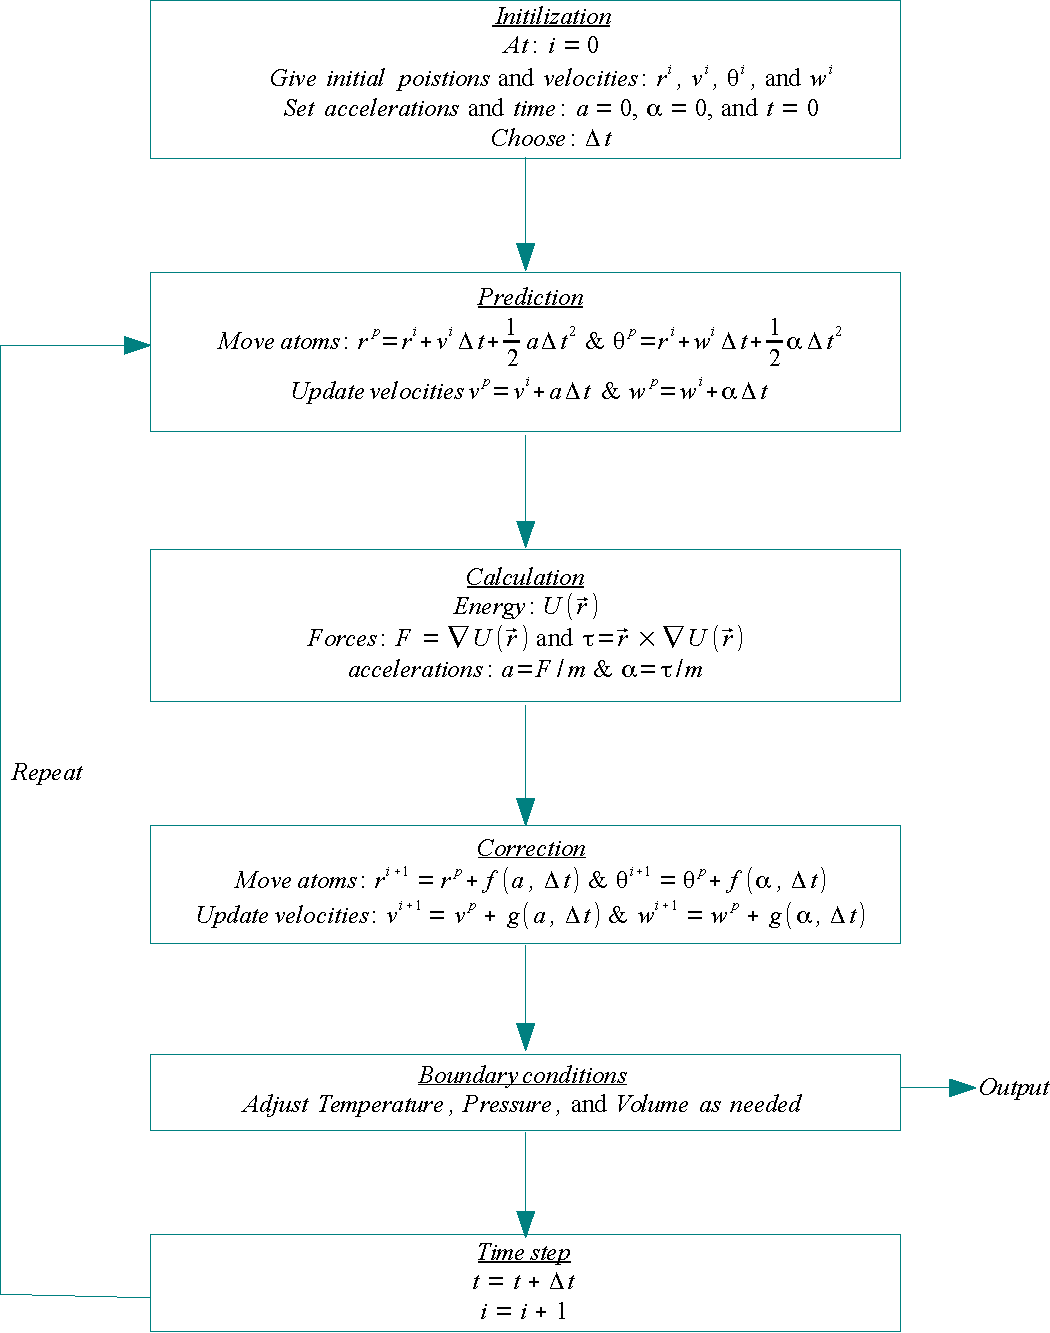
\includegraphics[width = \linewidth]{MD_flowchart.pdf}}
    \caption{Schematic figure showing the step-by-step process in Molecular dynamics simulation.}% where $r, v, \; \mathrm{and}\; a$ are linear position, velocity, and acceleration. and $%theta, %omega, \;\mathrm{and}\; %alpha$ .}are angular position, velocity, and acceleration respectively.% Similarly, $U, F, and %tau$ are energy, force, and torque respectively. The functions $f$ and $g$ evaluates correction factor for position and velocity using acceleration and time step.}
    \label{fig:MD}
  \end{center}
\end{figure}

In a MD simulation, all molecules are initialized by assigning their initial positions and velocities using appropriate boundary conditions. Molecules are usually initialized in such a way so that system does not take too long time to reach equilibrium. Before moving a molecule in the system, the computer must evaluate force and the potential energy contributed by intramolecular interactions as well as intermolecular interactions. The potential energy of the molecule in the system can be written as:
\begin{equation}
U(\mathbf r) = \overbrace{U_{bond} + U_{bend} + U_{torsion}}^{Intramolecular\; interactions} + \overbrace{U_{electrostatic} + U_{van\;der \;Waals}}^{Intermolecular\;interactions} + ...
\label{eq:potential}
\end{equation}   
The force and torque acting on the molecule can be calculated using following equations:

\begin{subequations}
\begin{gather}
\mathbf F = \nabla_r U(\mathbf r, \hat{u}) \\
\mathbf {\mathbf{\tau}} = \mathbf r \times \nabla_r U(\mathbf r, \hat{u}),
\end{gather}
\label{eq:forceTorque}
\end{subequations}
where $\hat{u}$ is the orientation of the molecule and the evaluation of force and torque depends on the direction of orientation for the point multipoles. The force and torque are required to propagate the dynamics to the molecule at a given time step. The same process can be repeated for every molecule in the system. Once every molecule in the system is moved forward a time-step, their positions and velocities are adjusted according to applied boundary conditions (i.e temperature, pressure, volume, etc are adjusted). After adjusting positions and velocities, we can recalculate the potential energy for each molecule and repeat same process until the simulation completes the allowed simulation time.
 
In MD simulations, the intermolecular interactions are the most expensive part of simulation. Among them, the van der Waals interactions are short-range interactions and are often described by Lennard-Jones (LJ) potential:

\begin{equation}
U_{LJ}(r) = 4\epsilon \left[\left(\frac{\sigma}{r} \right)^{12} - \left(\frac{\sigma}{r} \right)^6\right],
\label{eq:LJ}
\end{equation}
where $\sigma$ is diameter of a molecule and $\epsilon$ determines well depth of the attractive potential. The $1/r^6$ in the equation~\ref{eq:LJ} is short-ranged. The $1/r^{12}$ repulsive part of the  LJ potential prevents two or more molecules from occupying the same position. The electrostatic interactions are considered long-range interactions e.g. charge-charge interactions between molecules can be described by Coulomb's law: 

\begin{equation}
U_{electrostatic}(r) = \frac{1}{4\pi \epsilon_o}\frac{q_1 q_2}{r}.
\label{eq:Coulomb}
\end{equation}
Electrostatic interactions decay much slower with the distance. For charge-charge, they fall off as $ \frac{1}{r}$. If the lowest order moment in the molecule is a dipole, the electrostatic interaction will falls off by ${1}/{r^3}$. Even if the lowest order moment in molecule is a quadrupole, the electrostatic interaction will decay by ${1}/{r^5}$ which is longer range than LJ interaction. Since the electrostatic interaction decays slowly, we need to consider a large number of molecules around it to capture physical behavior due to interactions. Consideration of interactions with large number of molecules is not computationally efficient. The most important challenge in the molecular dynamics communities have been to capture right electrostatic behavior of a molecule considering only its interaction with a small number of neighboring molecules. There have been many efforts to develop efficient and accurate algorithms to evaluate electrostatic interaction in molecular simulation, which will be discussed in detail in section~\ref{sec:ElectMethod}.  

%The main purpose of our research is developing accurate and efficient electrostatic interaction methods considering small number of molecules around a given molecules.  
 
\subsection{Peridic Boundary Condition (PBC)}
Real liquid systems consist of very large number of molecules. But for computational efficiency, only a small number of particles ($\sim 10^3$) are usually considered in molecular simulations. On the other hand, if we want to study and predict bulk properties of the material using small number of molecules, a large fraction of molecules will be near the edge of the sample, contributing a huge surface effect. To eliminate surface effects, Periodic Boundary Conditions (PBC) have long been employed in various molecular simulations.\cite{Born1912}
In PBC, the simulation box is replicated throughout the space to form an infinite lattice. In the course of simulation, if a molecule moves in the central box, its images in replicated boxes will also move in the similar fashion. Similarly when a molecule leaves the central box, one of its images will enter the box through opposite face to conserve total number of particle in a central box (see figure~\ref{fig:PBC}). Therefore the system acts like there is no wall at the boundary of the central box and eliminates the surface effect in the computation. If we want to evaluate potential energy of a molecule, we can consider its interactions with nearest molecules or images using the minimum image convention.\cite{Allen04} Even for minimum image convention, we need to calculate large number of pairwise distances at every time step. Consider a system of N molecules, the potential energy of $i^{th}$ molecule we need to find its distances $r_{ij}$ with every $j^{th}$ molecules or images in the system. Therefore in total we need to calculate $\frac{1}{2} N (N-1)$ number of distinct distances at every time-step, which can make the computation very expensive. 

  
\begin{figure}[tpb]
  \begin{center}
    \centerline{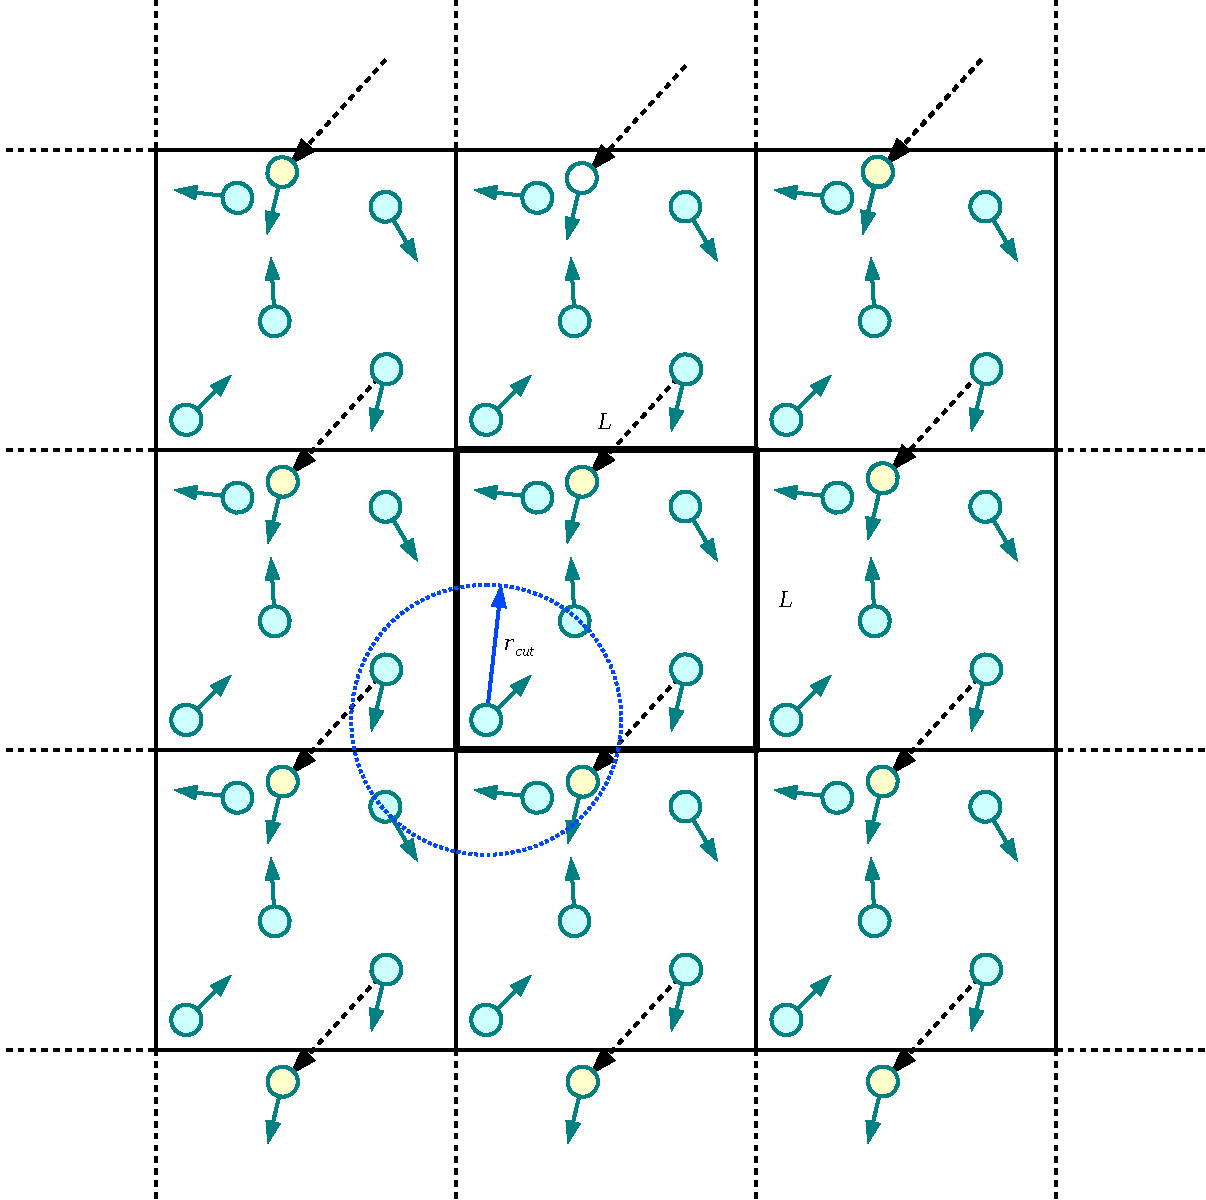
\includegraphics[width = \linewidth]{PBC.pdf}}
    \caption{Periodic Boundary Condition for two dimensional (2D) molecular system. The central 	box is outlined using thicker line and replicated throughout the plane to form a 2D lattice. Usually in molecular simulations, the potential energy of the molecule is evaluated considering its interactions with the molecules or their images located in the spherical cutoff region as shown in blue dotted-circle.}
    \label{fig:PBC}
  \end{center}
\end{figure}

\subsection{Spherical truncation and Neighbor lists }
If we assume the interaction between molecules is short-ranged, we can select small region around the molecule and consider that molecule only interacts with other molecules within that region. Often simulations use small cutoff regions around the molecule in order to make the MD simulation efficient. Beyond the cutoff region there is no interaction between the molecules. Consider a system of $N$  molecules with box size $L$. If PBC is employed, $r_{cut}$ should be less than $L/2$ in the molecular  simulation. If $r_{cut} > L/2$, a molecule may interact with another molecule as well as its own image at the same time, which can lead to spurious correlations in molecular dynamics simulation. The spherical truncation implemented in PBC is shown in figure~\ref{fig:PBC}. 

But evaluating all pair distances $r_{ij}$ at every time step for determining whether or not a particular molecule is within cutoff region makes simulation computationally expensive. Therefore cutoff sphere $r_{cut}$ is surrounded by the another larger sphere of radius $r_{list}$ as shown in figure~\ref{fig:neighbourList}. At the beginning of the simulation a list of the molecules, the neighbour list, is constructed around each molecule. For a few time steps, only the molecules in the neighbour list are selected to check whether or not molecule is within the cutoff sphere. After a few time steps, the neighbour list is reconstructed by evaluating pair distances between every molecules. This reconstruction time is mainly determined by the dynamics of the molecules in the simulation.  
\begin{figure}[tpb]
  \begin{center}
    \centerline{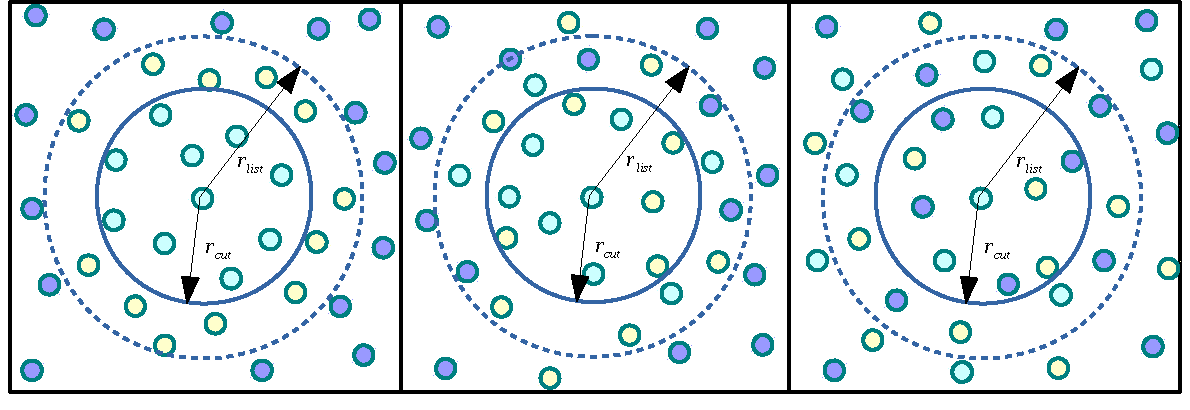
\includegraphics[width = \linewidth]{neighbourList.pdf}}
    \caption{Region of neighbor list around the cutoff sphere. Molecules in the cutoff region, neighbour list, and outer region are indicated by green, yellow, and violet circles respectively. The neighbour list  should be reconstructed before molecules in the outer region starts to penetrate the cutoff region.}
    \label{fig:neighbourList}
  \end{center}
\end{figure}


\section{Monte Carlo (MC) Simulation}
We need to sample a large number of different configurations to study any physical and statistical properties of the system. These configurations must take into account the ensemble being simulated. The Monte Carlo method uses probabilistic sampling of the system to generate representative configurations of the system. Each configuration depends only upon its predecessor but does not depend on the all the other configurations that were visited previously. For a canonical system, the probability of obtaining a given configuration is given by Boltzmann factor, $\mathrm{exp}(-{\Delta E}/{k_B T})$. Metropolis \textit{et.al} developed the selection criteria for acceptance of the subsequent configuration of the system. \cite{Metropolis53} According to their method, the new configuration of the system is accepted either  $\Delta E < 0$ or  $e^{-\frac{\Delta E}{k_B T}} > r$, where $r$ is the random number between 0 and 1. The evaluation of the potential energy difference between subsequent configurations, $\Delta E$, is very important in the MC simulation. For computational efficiency, this method also utilizes cutoff region $r_{cut}$ as well as periodic boundary condition to calculate electrostatic interaction. Therefore developing an efficient and accurate electrostatic interaction method has always been subject of interest in the MC community. 

\section{Electrostatic Methods}
\label{sec:ElectMethod}
Consider a system of $N$ particles in a cubic box of length $L$  replicated infinitely in 3D-space. The electrostatic potential energy for a particle with charge $q_i$ and position $r_i$ is given by
\begin{equation}
U_i =  \sum_n{}^{'}{ \sum_{j=1}^N {\frac{q_i q_j}{\lvert {\mathbf{r}_i-\mathbf{r}_j + \mathbf{n}L}\rvert}}},
\label{eq:electrostatic}
\end{equation}
where $q_j$ represents all other charges located at position $\mathbf{r}_j$ or in periodic replica and $\mathbf{n}$ is the cell-coordinate vector, $\mathbf{n}L = n_1 L \;\hat{x} + n_2 L\;\hat{y} + n_3 L\;\hat{z}$, where integers $n_1,n_2, \text{and}\; n_3$ number cells along the $x$, $y$, and $z$ directions and vary from 0 to $\infty$. The prime in the first sum indicates that $i =j $ should be ignored for the central box, i.e. $n = 0$. The factor ${1}/({4\pi\epsilon_o})$ has been dropped in the equation~\ref{eq:electrostatic} for simplicity. The total potential energy of the system can be calculated as,
\begin{equation}
U = \sum_{\substack{i=1 \\ i\neq j}}^N{U_i} = \frac{1}{2}\sum_n{}^{'}{\sum_{i=1}^N { \sum_{j=1}^N {\frac{q_i q_j}{\lvert {\mathbf{r}_i-\mathbf{r}_j + \mathbf{n}L}\rvert}}}},
\label{eq:totalElectrostatic}
\end{equation}
where factor of ${1}/{2}$ in the second part of the equation~\ref{eq:totalElectrostatic} is due to removal $i \neq j$ in the summation.
 
As we know the electrostatic interaction is a long-range interaction which is time consuming. On the other hand the potential energy evaluated using equation~\ref{eq:electrostatic} converges conditionally to the correct value depending on the order of summation taken into account during  calculation.\cite{Allen89} Therefore there have been many efforts to reduce computational cost and remove its conditionally convergent behavior.  

\subsection{Ewald Method}
The Ewald method was originally proposed by \texit{Ewald} in 1921 to evaluate electrostatic interactions in PBC. In this method, the electrostatic interaction  can divided into two rapidly converging real and reciprocal space sums as well as a constant self-term. \cite{Toukmaji96} Since  $\mathrm{erf}(x) + \mathrm{erfc}(x) = 1$ we can write equation~\ref{eq:totalElectrostatic} as,

\begin{equation}
U = \frac{1}{2}\sum_n^{'}{\sum_{i=1}^N { \sum_{j=1}^N {q_i q_j}}}\frac{\mathrm{erfc}(\alpha r_{ij,n})+\mathrm{erf}(\alpha r_{ij,n})}{r_{ij,n}}.
\label{eq:errorFuncElectrostatic}
\end{equation} 
The real-space term~\ref{eq:ewald1} in Ewald method is obtained by taking complementary error function term in the equation~\ref{eq:errorFuncElectrostatic}. Similarly reciprocal-space part~\ref{eq:ewald2} can be obtained by taking Fourier transform of the error function term in equation~\ref{eq:errorFuncElectrostatic}. The self-term present in the equation removes artificial interactions of the charge with its own images located in the periodic replicas. 

\begin{subequations}
\begin{gather}
U_{real} = \frac{1}{2} \sum_{i,j}^{N}{\sum_{n}^{'}{{q_i q_j}\frac{\mathrm{erfc}(\alpha r_{ij,n})}{r_{ij,n}}}}, \label{eq:ewald1}\\
U_{reciprocal} = \frac{1}{2\pi V}\sum_{i,j}^{N}{\sum_{\mathbf{m} \neq 0}\frac{\exp(-(\pi \mathbf{m}/\alpha)^2 + 2\pi i \mathbf{m}\cdot{\mathbf{r}_{ij})}}{\mathbf{m}^2}},\label{eq:ewald2} \\
U_{self} = -\frac{\alpha}{\sqrt{\pi}} \sum_{i =1}^{N} {q_i}^2 ,\label{eq:ewald3}
\end{gather}
\end{subequations}
where $V$ is the volume of the simulation box, $\mathbf{m}$ is a reciprocal-space vector, and $\alpha$ is a damping parameter which determines the rate of convergence in the real and reciprocal space. 
 
Physically each point charge in the system can be assumed to be surrounded by a Gaussian distribution of equal magnitude but oppositely-signed charge (see figure~\ref{fig:Ewaldsum}) with density,

\begin{equation}
\rho_i (r) = q_i \left(\frac{\alpha}{\sqrt{\pi}}\right)^3 \exp(-\alpha^2 r^2),
\label{eq:chargeDistribution}
\end{equation}
where $\alpha$ is a damping parameter determines the distribution of the charge, and $r$ is the distance from the center of distribution. The imposed charge distribution around a charge screens the interactions between the charges making the effective interaction  short ranged and therefore converges rapidly with distance. These Gaussian distributions are counteracted by other Gaussian distributions of charge having same magnitude but opposite sign as shown in figure~\ref{fig:Ewaldsum}. \cite{Toukmaji96} The sum of potential energy due to second type of charge distributions converges in reciprocal space. 

\begin{figure}[tpb]
  \begin{center}
    \centerline{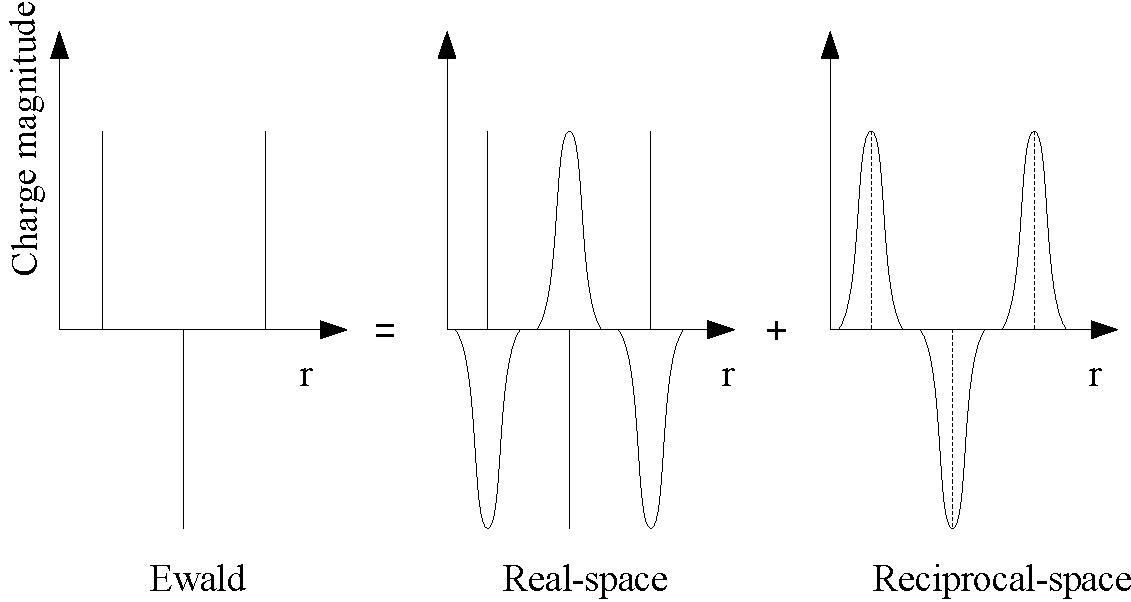
\includegraphics[width = \linewidth]{Ewaldsum.pdf}}
    \caption{In the Ewald method each point charge is surrounded by a Gaussian distribution of equal and oppositely-signed charge, evaluated in real-space. These Gaussian distributions are compensated by the opposite-singed Gaussian distribution of the charges calculated in reciprocal-space }
    \label{fig:Ewaldsum}
  \end{center}
\end{figure}

In the minimum image convention scheme, each particle can interact with its nearest particles or their image, the total number of interactions is $\frac{1}{2}N(N-1)$ in Ewald method. Therefore the algorithmic complexity for the Ewald method is $O(N^2)$. Recerz and Jacobs suggested that by choosing proper simulation parameters and minimum image convention schemes we can make reciprocal potential very small as compared to real-space potential so that can be ignored.\cite{Jacobs92} However this method is only applicable for a larger system but contribution of the reciprocal-space sum might not small for all systems, therefore is not recommended for general MD simulations. Perram \textit{et al.} subdivided each simulation box into $m \times m \times m$ sub-boxes and selected damping parameter $\alpha = m \sqrt{-\log(\delta)}$ , where $\delta$ is the relative error constant for neglecting the maximum term in the real-space sum, and using this technique they were able to reduce computational time   to $O(N^{3/2})$.

\subsection{Fourier-based Ewald Methods}
The Ewald method has been further modified using Fast Fourier transforms (FFT) to reduce complexity to $O(N\log(N))$. In these methods, charges are interpolated onto a 3D grid and the reciprocal sum is evaluated using FFTs. The particle-particle particle-mesh Ewald (PPPME) and particle-mesh Ewald (PME) methods are two widely-used Fourier-based Ewald methods. 

\begin{figure}[tpb]
  \begin{center}
    \centerline{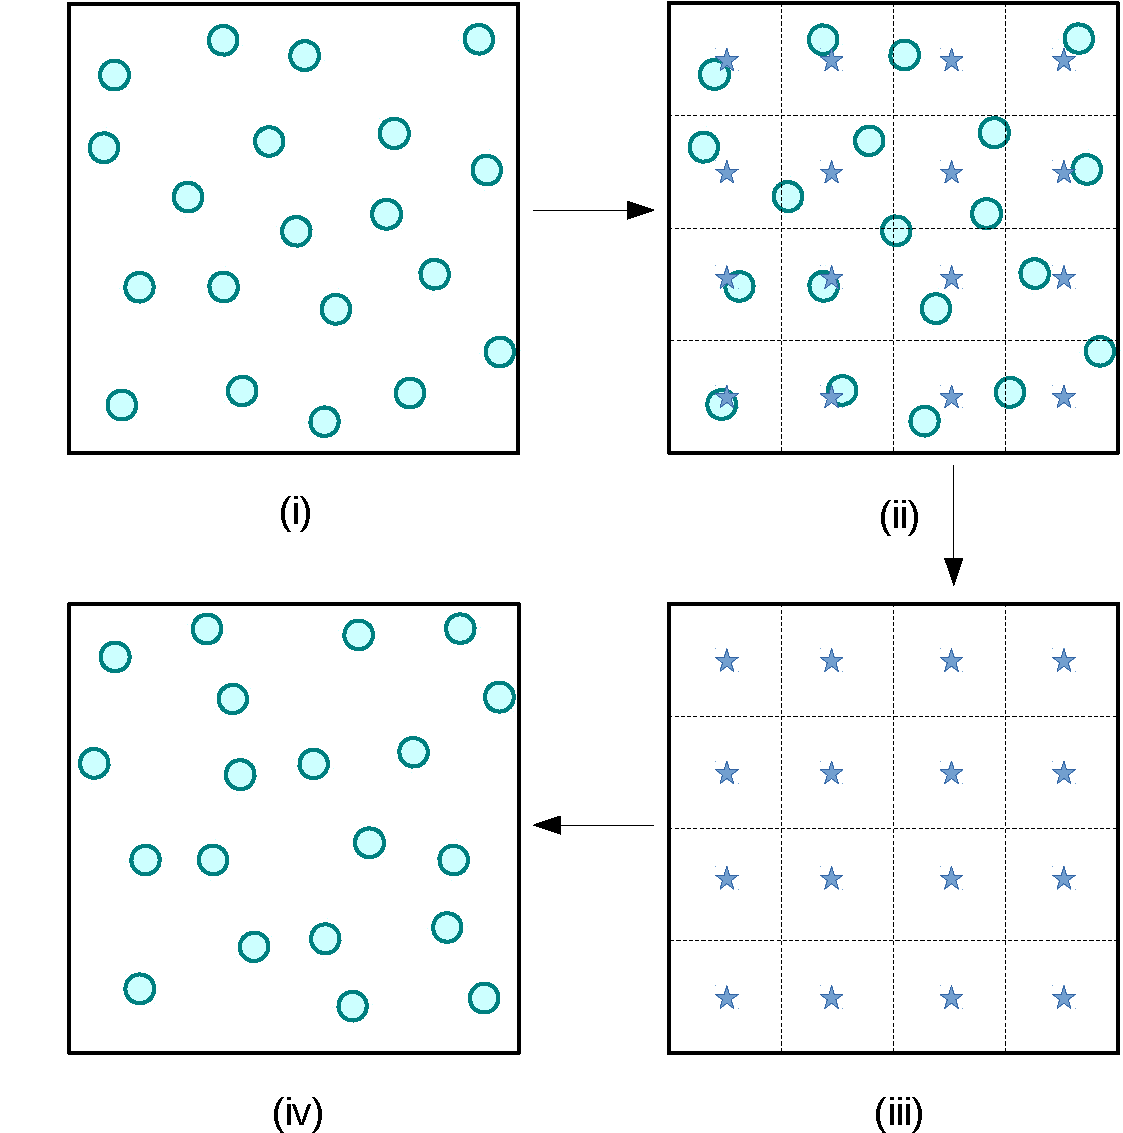
\includegraphics[width = \linewidth]{PM_method.pdf}}
    \caption{Schematic diagram for Fourier-based Ewald methods where green circle represents charge and blue star denotes grid point. In the figure, (i) a system of charges, (ii) charges mapped with grid points, (iii) force evaluated at the grid points, and (iv) force mapped back to the particles and their positions and velocities are updated. }
    \label{fig:PPPME}
  \end{center}
\end{figure}
\subsubsection{Particle-Particle Particle-Mesh Ewald (PPPME)}
\label{subsec:PPPME}
The PPPME method was originally developed by Hockmney and Eastwood \cite{Hockney88} and extended  by Luty \textit{et al.}.\cite{Luty94} and Rajagopal \textit{et al.} \cite{Rajagopal94} In this method, the electrostatic interaction is divided into short-ranged real-space and long-ranged reciprocal-space sums. The charges in the system are approximated as uniformly decreasing spherical charge density. The short-ranged potential within the cutoff radius $r < r_{cut}$ is calculated using electrostatic interactions between charge distributions. To calculate the long-ranged potential, first of all charges are assigned to the 3D grid as shown in figure~\ref{fig:PPPME} and transformed to the Fourier space for evaluating electrostatic potential. Since charges are assigned to the grid, it is very efficient to calculate electrostatic interactions in reciprocal space. Once the potential energy is evaluated, an inverse Fourier transformation is applied to calculate energy in real-space and it is numerically differentiated to get the force acting on the grid. Finally the electrostatic force (or energy) can be interpolated from the grid onto the particle locations to obtain actual force acting on the particle.

Although PPPME has complexity of $O(N \mathrm{log}N)$, for computational accuracy, we either need to refine the mesh or use better interpolation techniques, both of which are computational expensive. In addition to this, using numerical differentiation to calculate forces may introduce errors in the calculation. Therefore higher order differentiation schemes are often used in force calculations. In order to get optimal performance, all of the parameters; charge-distribution, interpolation technique, and differentiation schemes must be properly selected for a given system making  parameter choices system specific. \cite{Toukmaji96}

\subsubsection{Particle-Mesh Ewald (PME)}
\label{subsubsec:PME}
This method is the modification of the PPPME method, in which the potential energy is divided into real-space and reciprocal-space sums. The charge is represented by the Gaussian distributions of charge. In this method, the real-space sum within the cutoff sphere is evaluated using actual electrostatic interactions between charges whereas the reciprocal sum is calculated in Fourier space using the idea of 3D grid as explained in the PPPME method. Unlike PPPME, this method evaluates force analytically, differentiating electrostatic energy at a given grid point reducing memory requirement significantly. This method also has $O(N\mathrm{log}N)$ algorithmic complexity and uses interpolation to map back electrostatic force from grid to the particle's location. Therefore users of this method need to discover optimal interpolation schemes to obtain excellent speed and accuracy for a simulation, making this method system dependent.

\subsection{Real Space Methods}
Before discussing the real space methods, the fundamental property of the electrostatic interactions in condensed phase environments should be considered. The electrostatic interaction between two charged particles decays as $1/r$. But molecular systems are usually composed of an equal number of positive and negative charges. Thus the range of interaction between a particular charge and rest of the charges in the system are different than the interaction between two bare charges. Consider a one dimensional (1D) crystal lattice composed of positive and negative charges. The potential energy of a particular ion can be considered as a sum of interactions with positive and negative ion pairs as shown in figure~\ref{fig:schematic}(a). Mathematically the potential energy for 1D crystal with alternating charges is given by a Madelung sum,

\begin{equation}
\begin{split}
U^{Mad} & = -2q_iq_j\left(\frac{1}{a}-\frac{1}{2a}\right)-2q_iq_j\left(\frac{1}{3a}-\frac{1}{4a}\right)-2q_iq_j\left(\frac{1}{5a}-\frac{1}{6a}\right) + ... \\
		& = -\left(\frac{ 2q_iq_j}{(1.414)^2a}\right)-\left(\frac{2q_iq_j}{(3.464)^2a}\right)-\left(\frac{2q_iq_j}{(5.477)^2a}\right) +...
\end{split}
\label{eq:1D}
\end{equation} 
 
\begin{figure}
  \centering
  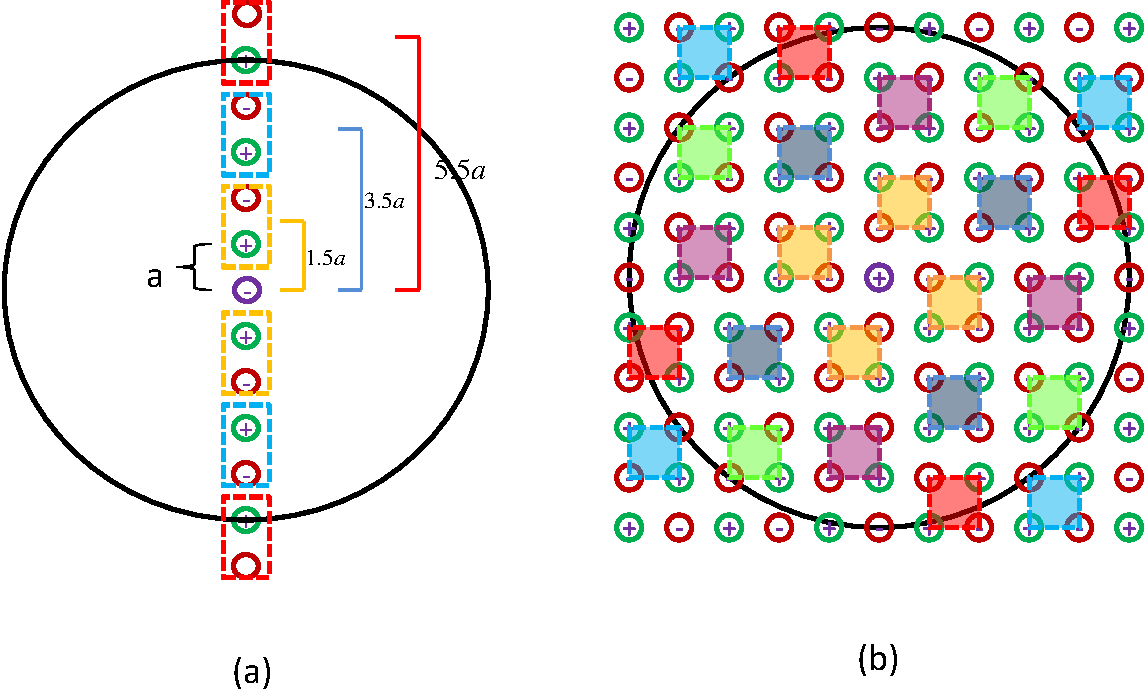
\includegraphics[width=\linewidth]{1D_2DCrystal.pdf}
  \caption{Schematic diagram showing grouping of ions in (a) 1D (b) 2D crystals. The interaction of the central ion with the group of ions decays faster than $1/r$. The direct spherical truncation breaks the ordering of the ions at the cut off sphere providing a net charge within the cutoff sphere. The breaking of the charge ordering increases with the crystal dimension resulting in a large net charge in the higher dimensional crystal.}
   \label{fig:schematic}
\end{figure}

If we consider all 3 terms in the equation~\ref{eq:1D} and compare their distances with the distance between central ion and group of ions as shown in figure~\ref{fig:schematic}(a), we clearly see that the interaction energy of a single ion with the pairs converges faster than ($1/r$). Similarly, in a two dimensional (2D) lattice, the potential energy of an ion can be described as a sum of positive and negative four body groups as seen in figure~\ref{fig:schematic}(b). The interaction energy between an ion and group of four ions decays much faster than the charge-charge interaction. For a three-dimensional (3D) crystal, the potential energy of an ion can be considered as due to its interaction with the group of eight ions forming a cube. From this generalization, we can conclude that the electrostatic interaction energy for an ion in the crystalline system is a short-ranged as compared to charge-charge interaction. Therefore, even the relatively small systems should be able to represent bulk long-ranged interactions.


In order to reduce the computational expense of a molecular dynamics simulation, interactions between particles are only considered if the particles exist within a cutoff distance $r_c$, of one another. We first consider how the energy of a system behaves if we truncate the interactions at the cutoff radius.  Figure~\ref{fig:energyVsCutoff} shows (black line) that the electrostatic potential energy does not converge to the Madelung energy upon increasing the cutoff radius for the direct truncation. On the other hand the energy is found to be closer to the Madelung constant when the net charge within the cutoff radius is zero (figure~\ref{fig:energyVsCharge}). This oscillation in the potential energy is due to the breaking in charge ordering on the surface of the cutoff sphere which results in a net charge within the cutoff sphere. The size of the net charge is proportional to the dimension of the crystal. Although the interaction energy is short ranged,  the direct truncation results in severe oscillation in energy for 3D crystal as shown in figure~\ref{fig:energyVsCutoff}. Dipolar (or quadrupolar) crystals are also formed by ordering of the dipolar (or quadrupolar) molecules. Therefore similar oscillatory behaviour in the potential energy is due to the breaking of the ordering of dipoles (or quadrupoles) on the surface of the truncated sphere. Even in liquids there is local ordering of the molecules due to electrostatic interaction and similar oscillatory behaviour in the electrostatic potential has been seen in direct truncation approaches.

\begin{figure}[tpb]
  \begin{center}
    \centerline{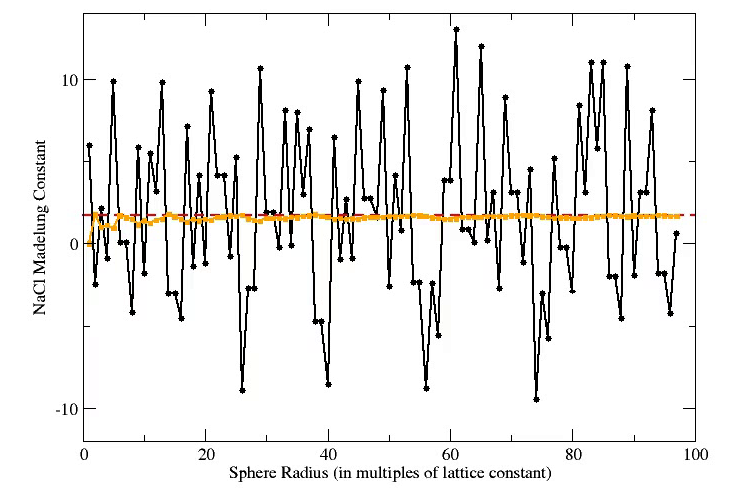
\includegraphics[width = \linewidth]{energyVsCutoff.png}}
    \caption{Convergence of the lattice energy constants for a 3D NaCl crystal as a function of cutoff radius for the direct (hard) cutoff method (black line). The orange line in the figure is for charge neutralized cutoff sphere (when image charge placed on the surface of the cutoff sphere). The red dotted line represents Madelung energy for NaCl crystal}
    \label{fig:energyVsCutoff}
  \end{center}
\end{figure}

\begin{figure}[tpb]
  \begin{center}
    \centerline{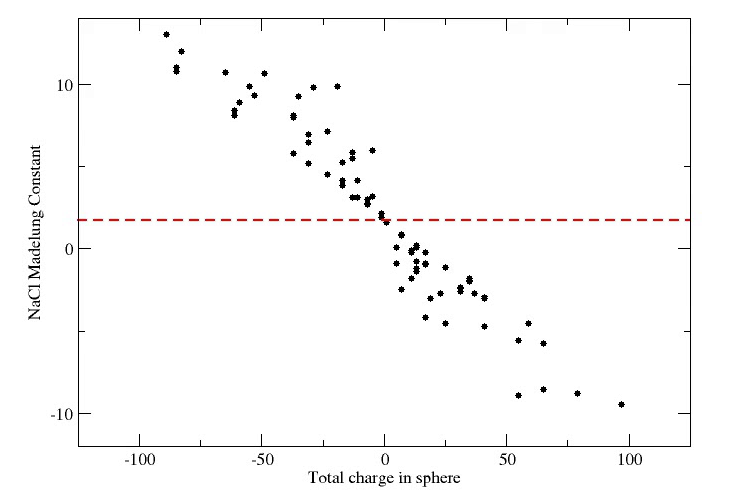
\includegraphics[width = \linewidth]{energyVsNetcharge.png}}
    \caption{Convergence of the lattice energy constants for the NaCl crystal as a function of net charge within a cutoff sphere. The red dotted line represents Madelung energy for NaCl crystal}
    \label{fig:energyVsCharge}
  \end{center}
\end{figure}
Wolf \textit{et al} \cite{Wolf99} proposed the idea of placing an image charge on the surface of cutoff sphere for every charge found within the sphere. The image charges should have opposite charge of those found within the sphere guaranteeing charge neutralization  within the cutoff sphere.\cite{Wolf99} This charge neutralization converges the potential energy to the correct Madelung energy as shown in figure~\ref{fig:energyVsCutoff} (orange line). In molecular dynamics (MD) simulations, the energy, force and torque should approach zero as the distance between molecules approaches the cutoff radius  in order to conserve total energy. However Wolf's forces and torques derived from the potential do not go to zero at the cutoff radius, which makes it inappropriate to use in MD simulations. More recently, Zahn \textit{et al.} and Fennell and Gezelter proposed the damped shifted force (DSF) potential, which incorporates Wolf's approach of image charges while ensuring the forces and torques approach zero at the cutoff radius.\cite{Zahn02, Gezelter06} Fukuda has also recently been successful with the neutralization of higher order moments in a system of point charges.\cite{Fukuda13}

Real-space methods scale linearly with system size, are system-independent, and applicable a variety of condensed phase environments. Therefore we selected real-space methods for extending to higher-order charge-multipoles. In our research, we have generalized Wolf's shifted potential (SP) to the higher order electrostatic multipoles. We have also developed the gradient shifted force (GSF) and Taylor shifted force (TSF) potentials which are the natural extension of the damped shifted force (DSF) for higher order charge-multipoles. In the following chapter 2, I will discuss the development of the SP, GSF, and TSF methods and evaluate the energy constants for various dipolar and quadrupolar crystals using newly developed methods and compare with analytical results.\cite{Lamichhane14_I} 